\documentclass{article} 
\usepackage{tikz} 
\begin{document} 
\begin{center} 
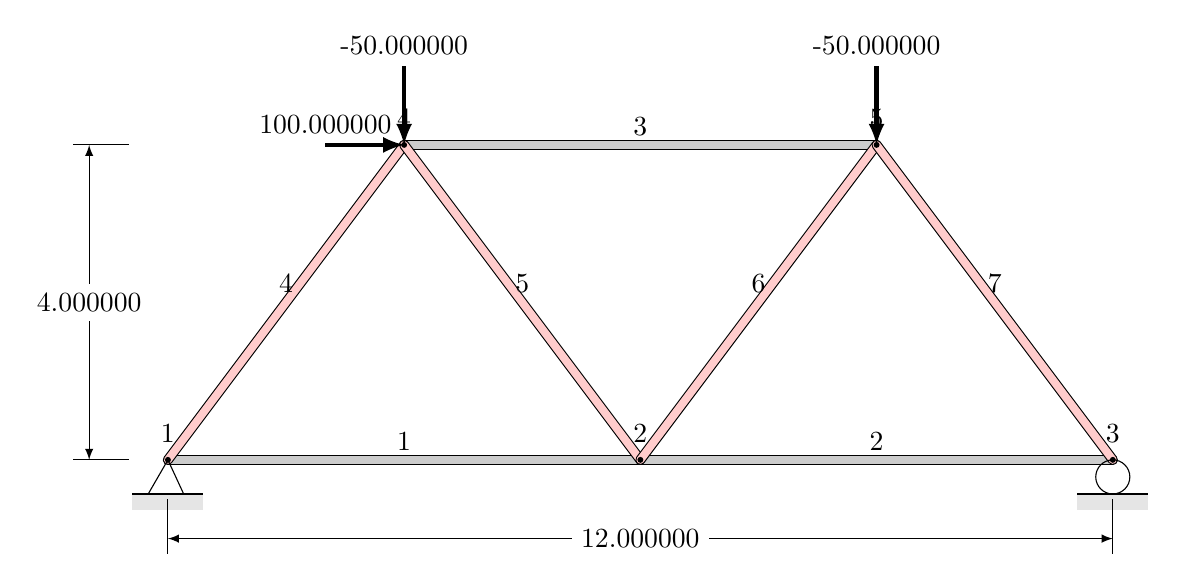
\begin{tikzpicture} 
% estilos de linea y relleno 
\tikzstyle{carga} = [ultra thick,latex-]  
% definicion apoyo de segundo genero 
% #1: ubicación del apoyo 
% #2: angulo de rotacion 
 \newcommand{\apoyoseg}[2]{ 
\coordinate (O) at #1; 
\begin{scope}[rotate around={#2:(O)}] 
\fill [black!10](O) ++(-0.45,-0.433013) rectangle ++(0.9,-0.2); 
\draw [thick] (O) ++(-0.45,-0.433013) -- ++(0.9,0); 
\draw (O) -- ++(-0.25,-0.433013) -- ++(0.45,0) -- cycle; 
\end{scope} 
 } 
% definicion apoyo de primer genero 
% #1: ubicación del apoyo 
% #2: angulo de rotacion 
 \newcommand{\apoyopri}[2]{ 
\coordinate (O) at #1; 
\begin{scope}[rotate around={#2:(O)}] 
\fill [black!10](O) ++(-0.45,-0.433013) rectangle ++(0.9,-0.2); 
\draw [thick] (O) ++(-0.45,-0.433013) -- ++(0.9,0); 
\draw (O) ++(0,-0.216506) circle (0.216506); 
\end{scope} 
 } 
% definicion carga puntual 
% #1: ubicación de la carga 
% #2: rótulo de la carga 
% #3=1: carga positiva, #3=-1: carga negativa 
% #4=1,#5=0: carga en x, #4=0,#5=1: carga en y 
% #6=0: carga entrando al nudo, #6=1: carga saliendo del nudo 
% #7: ubicación del rótulo de la carga 
\newcommand{\cargapun}[7]{ 
\path #1 ++(#6*#4,#6*#5) coordinate (O); 
\draw [carga] (O) -- ++(-1.0*#3*#4,-1.0*#3*#5) 
node [#7] {#2}; 
 } 
% cota horizontal 
% #1: coordenada punto inicial () 
% #2: coordenada punto final () 
% #3: rotulo de la cota 
% #4: separación entre puntos y cota 
% #5: separación entre puntos y inicio de marcas 
% #6: separación entre cota y fin de marcas 
\newcommand{\cotahori}[6]{ 
\path #1 ++(0,#4) coordinate (A); 
\path #2 ++(0,#4) coordinate (B); 
\draw [latex-latex] (A) -- (B) 
node [midway,fill=white] {#3}; 
\path #1 ++(0,#5) coordinate (C); 
\path #1 ++(0,#4+#6) coordinate (D); 
\draw (C) -- (D); 
\path #2 ++(0,#5) coordinate (C); 
\path #2 ++(0,#4+#6) coordinate (D); 
\draw (C) -- (D); 
 } 
% cota vertical 
% #1: coordenada punto inicial () 
% #2: coordenada punto final () 
% #3: rotulo de la cota 
% #4: separación entre puntos y cota 
% #5: separación entre puntos y inicio de marcas 
% #6: separación entre cota y fin de marcas 
\newcommand{\cotavert}[6]{ 
\path #1 ++(#4,0) coordinate (A); 
\path #2 ++(#4,0) coordinate (B); 
\draw [latex-latex] (A) -- (B) 
node [midway,fill=white] {#3}; 
\path #1 ++(#5,0) coordinate (C); 
\path #1 ++(#4+#6,0) coordinate (D); 
\draw (C) -- (D); 
\path #2 ++(#5,0) coordinate (C); 
\path #2 ++(#4+#6,0) coordinate (D); 
\draw (C) -- (D); 
 } 
% dibujar elementos 
\tikzstyle{elem}=[double distance = 0.1cm,line cap=round]; 
\tikzstyle{elet}=[black,midway,above]; 
\tikzstyle{mat1}=[double=black!20]; 
\tikzstyle{mat2}=[double=red!20]; 
\tikzstyle{mat3}=[double=green!30]; 
\tikzstyle{mat4}=[double=blue!40]; 
\begin{scope} 
\draw[elem,mat1] (0.000000,0.000000)--(6.000000,0.000000) node[elet] {1}; 
\draw[elem,mat1] (6.000000,0.000000)--(12.000000,0.000000) node[elet] {2}; 
\draw[elem,mat1] (3.000000,4.000000)--(9.000000,4.000000) node[elet] {3}; 
\draw[elem,mat2] (0.000000,0.000000)--(3.000000,4.000000) node[elet] {4}; 
\draw[elem,mat2] (3.000000,4.000000)--(6.000000,0.000000) node[elet] {5}; 
\draw[elem,mat2] (6.000000,0.000000)--(9.000000,4.000000) node[elet] {6}; 
\draw[elem,mat2] (12.000000,0.000000)--(9.000000,4.000000) node[elet] {7}; 
\end{scope} 
% dibujar nudos 
\tikzstyle{nudo}=[fill=black]; 
\tikzstyle{nudt}=[above=0.1cm]; 
\def \r{0.03cm}; 
\begin{scope} 
\draw[nudo] (0.000000,0.000000) circle (\r) node[nudt] {1}; 
\draw[nudo] (6.000000,0.000000) circle (\r) node[nudt] {2}; 
\draw[nudo] (12.000000,0.000000) circle (\r) node[nudt] {3}; 
\draw[nudo] (3.000000,4.000000) circle (\r) node[nudt] {4}; 
\draw[nudo] (9.000000,4.000000) circle (\r) node[nudt] {5}; 
\end{scope} 
% dibujar apoyos 
\apoyoseg{(0.000000,0.000000)}{0} 
\apoyopri{(12.000000,0.000000)}{0} 
% dibujar cargas puntuales 
\cargapun{(3.000000,4.000000)}{100.000000}{1.000000}{1}{0}{0}{above} 
\cargapun{(3.000000,4.000000)}{-50.000000}{-1.000000}{0}{1}{0}{above} 
\cargapun{(9.000000,4.000000)}{-50.000000}{-1.000000}{0}{1}{0}{above} 
% dibujar cotas 
\cotahori{(0.000000,0.000000)}{(12.000000,0.000000)}{12.000000}{-1}{-0.5}{-0.2} 
\cotavert{(0.000000,0.000000)}{(0.000000,4.000000)}{4.000000}{-1}{-0.5}{-0.2} 
\end{tikzpicture} 
\end{center} 
\end{document} 
